%%%%%%%%%%%%%%%%%%%%%%%%%%%%%%%%%%%%%%%%%%%%%%%%%%%%%%%%%%%%%%%%%%%%%%%%%%%%%%
% Plik ten należy, co najmniej dwukrotnie, przetworzyć przy użyciu komendy 'pdflatex'
%
% Stanisław Polak, 25-01-2017
%%%%%%%%%%%%%%%%%%%%%%%%%%%%%%%%%%%%%%%%%%%%%%%%%%%%%%%%%%%%%%%%%%%%%%%%%%
%%%%%%%%%%%%%%%%%%%%%%%%%%%%%%%%%%%% Włączenie, domyślnego, trybu "beamer" 
%%%%%%%%%%%%%%%%%%%%%%%%%%%%%%%%%%%%%%%%%%%%%%%%%%%%%%%%%%%%%%%%%%%%%%%%%%
\documentclass[polish,xcolor=table,9pt,aspectratio=1610,hyperref={pdfpagemode=FullScreen}]{beamer} 
% Opcje:
% 	[polish]                            włączenie polonizacji
% 	[xcolor=table]                      włączenie możliwości kolorowania tabel - ładowanie pakietu ,,colortbl''
% 	[ascpectratio=1610]                 slajdy w proporcji 16:10, domyślnie 4:3
% 	[9pt]                              	podstawowy font ma mieć rozmiar '9pt', domyślna wartość to '11pt'. Dostępne wartości: 8pt, 9pt, 10pt, 11pt, 12pt, 14pt, 17pt, 20pt
% 	[hyperref={pdfpagemode=FullScreen}]	przeglądarka PDF ma automatycznie wyświetlać prezentację w trybie 'pełny ekran'

%%%%%%%%%%%%%%%%%%%%%%%%%%%%%%%%%%%%%%%%%%%%%%%%%%%%%%%%%%%%%%%%%%%%%%%%%%%%%%%%%%%%%% 
% Jeżeli chcesz otrzymać prezentacje w postaci materiałów drukowanych (dla słuchaczy),
% to należy zakomentować linię 8:  '\documentclass[...]{beamer}', 
% a odkomentować linię  23:'\documentclass[handout,...]{beamer}'
%%%%%%%%%%%%%%%%%%%%%%%%%%%%%%%%%%%%%%%%%%%%%%%%%%%%%%%%%%%%%%%%%%%%%%%%%%%%%%%%%%%%%% 
%%%%%%%%%%%%%%%%%%%%%%%%%%%%%%%%%%%% Włączenie trybu "handout" %%%%%%%%%%%%%%%%%%%%%%%
%%%%%%%%%%%%%%%%%%%%%%%%%%%%%%%%%%%%%%%%%%%%%%%%%%%%%%%%%%%%%%%%%%%%%%%%%%%%%%%%%%%%%% 
%\documentclass[handout,polish,xcolor=table,9pt,aspectratio=1610]{beamer} 

%%%%%%%%%%%%%%%%%%%%%%%%%%%%%%%%%%%%%%%%%%%%%%%%%%%%%%%%%%%%%%%%%%%%%%%%%%%%%%%
\usepackage[utf8]{inputenc}
\usepackage{polski}   %włączenie obsługi polskich liter
\usepackage{babel}    %aby zadziałała polonizacja 'beamera'
\usepackage{graphicx} %włączenie obsługi grafiki
\DeclareGraphicsRule{.pdftex}{pdf}{*}{}
\AtBeginPart{\frame{\partpage}} %Na początku każdej z części prezentacji, wyświetlaj jej tytuł
%%%%%%%%%%%%%%%%%%%%%%%%%%%%%%%%%%%%%%%%%%%%%%%%%%%%%%
% Komendy, które mają być wykonywane w trybie 'beamer'
%%%%%%%%%%%%%%%%%%%%%%%%%%%%%%%%%%%%%%%%%%%%%%%%%%%%%%
\mode<beamer>{ 
  %%%%%%%%%%%%%%%%%%%%%%%%%%%%%%%%%%%%%%%%%%%%%%%%%%%%%%%%%%%%%%%%%%%%%%%%%%%%%%%
  %'CambridgeUS' jest przykładowym stylem (wystrojem) - inne style można obejrzeć na stronie 
  % http://gknor.keep.pl/beamer/beamer_motywy.html
  % Zastosowany wystrój ma wpływ na wygląd struktury slajdu (nagłówki, stopki, rodzaje obramowania, itp.) jak i jego kolorystyki
  %%%%%%%%%%%%%%%%%%%%%%%%%%%%%%%%%%%%%%%%%%%%%%%%%%%%%%%%%%%%%%%%%%%%%%%%%%%%%%%
  % Na stronie https://github.com/polaksta/beamer-AGH można znaleźć styl AGH
  %%%%%%%%%%%%%%%%%%%%%%%%%%%%%%%%%%%%%%%%%%%%%%%%%%%%%%%%%%%%%%%%%%%%%%%%%%%%%%%
	\usetheme{CambridgeUS} %Określanie stylu (wystroju) prezentacji
	\usecolortheme{orchid} %Określanie schematu kolorów - zmiana kolorystyki slajdu
}
%%%%%%%%%%%%%%%%%%%%%%%%%%%%%%%%%%%%%%%%%%%%%%%%%%%%%%%
% Komendy, które mają być wykonywane w trybie 'handout'
%%%%%%%%%%%%%%%%%%%%%%%%%%%%%%%%%%%%%%%%%%%%%%%%%%%%%%%
\mode<handout>{
  \usepackage{pgfpages}
  \pgfpagesuselayout{4 on 1}[a4paper,border shrink=5mm,landscape] %Wynikowy dokument PDF będzie zawierał cztery slajdy na jednej stronie kartki formatu A4
  \usetheme{boxes} %Określanie stylu (motywu) prezentacji
  \addheadbox{structure}{\quad\insertsubsection\hfill\insertsection\hfill\inserttitle\qquad} %Określanie zawartości nagłówka kartki
  \addfootbox{structure}{\quad\insertauthor\hfill\insertframenumber\hfill\insertsubtitle\qquad} %Określanie zawartości stopki kartki
}
%%%%%%%%%%%%%%%%%%%%%%%%%%%%%%%%%%%%%%%%%%%%%%%
% Określamy tytuł, autora, afiliację  oraz datę prezentacji
% UWAGA, poniższe komendy tylko definiują treść slajdu tytułowego
% Jeżeli chcemy umieścić te informacje na slajdzie należy
% w ciele dokumentu umieścić komendę '\maketitle' lub '\frame{\titlepage}'
%%%%%%%%%%%%%%%%%%%%%%%%%%%%%%%%%%%%%%%%%%%%%%%
\title{Framework e-commerce}
\subtitle{Elastyczny szablon sklepu internetowego}
\author{Przemysław Magiera}
\begin{document}

%%%%%%%%%%%%%%%%%%%%%%%%%%%%%%%%%%%%%%%%%
%%%%% Slajd ze stroną tytułową %%%%%%%%%%
%%%%%%%%%%%%%%%%%%%%%%%%%%%%%%%%%%%%%%%%%
% Komenda \tilepage tworzy stronę tytułową na podstawie \title, \author, \institute oraz \date zawartych w preambule (patrz wyżej)
\frame{\titlepage}

\section{Wymagania}
\subsection{Współczesne frameworki e-commerce}

\begin{frame}{Wymagania współczesnego sklepu}
\begin{itemize}
\item<1-> łatwe dodawanie nowych funkcjonalności 
\item<1-> zarządzanie i możliwość konfiguracji każdej funkcjonalności
\item<1-> wydajny katalog produktowy mogący obsłużyć duży ruch
\item<1-> szybki i nieskomplikowany dostęp do informacji, której wymaga klient

\end{itemize}
\end{frame}


\section{Zastosowane rozwiązania}

\subsection{Dynamiczny panel administracyjny}
\begin{frame}{Dynamiczny panel administracyjny}
\begin{figure}
	\begin{center}
		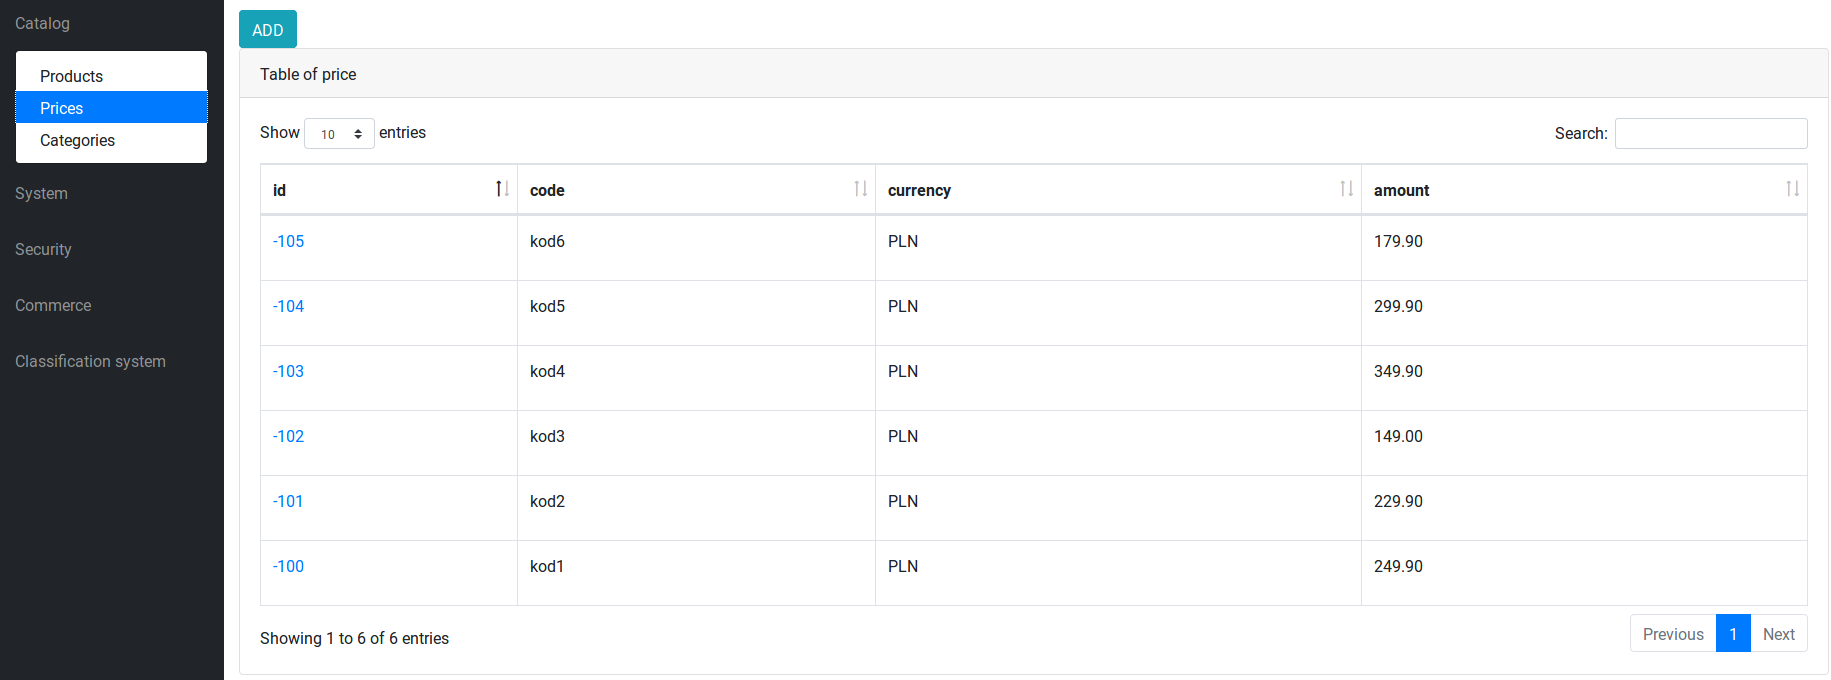
\includegraphics[scale=0.18]{admin-main.png}
	\end{center}
	\caption{{\color{black}Widok panelu administracyjnego}} 
\end{figure}
	\begin{itemize}
		\item<1-> konfigurowalne menu administracyjne
		\item<1-> generowana tabelka dla każdej encji danego rodzaju np. kategorii 
		\item<1-> generowany formularz edycji dowolnej encji
		\item<1-> mechanizm zarządzania relacjami dowolnej klasy np. dzieci kategorii
	\end{itemize}
\end{frame}

\begin{frame}{Panel administracyjny}{Dynamiczne menu}
\begin{columns}
	\begin{column}{0.5\textwidth}
		\begin{itemize}
			\item<1-> Menu w panelu jest oparte na dwóch tabelach \texttt{admin-menu-item} oraz \texttt{admin-menu-group}
			\item<1-> AdminMenuItem i AdminMenuGroup to też encje, więc konfigurujemy widok panelu admina
			\item<1-> efekt jest taki, że każdą encję, którą dodamy do tych tabel będziemy mogli zarządzać z poziomu panelu admina
		\end{itemize}
	\end{column}
	\begin{column}{0.5\textwidth}
			\begin{figure}
				\begin{center}
					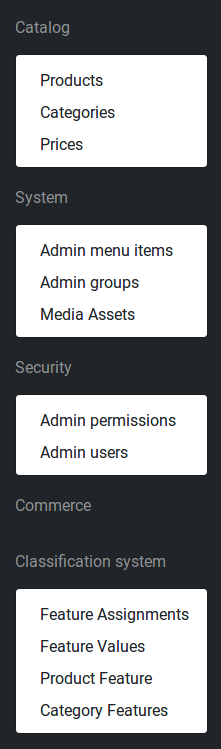
\includegraphics[scale=0.2]{menu.png}
				\end{center}
				\caption{{\color{black}Menu w panelu administracyjnym}} 
			\end{figure}
	\end{column}
\end{columns}
\end{frame}

\begin{frame}{Panel administracyjny}{Zarządzanie funkcjonalnościami, które mogą zostać dopisane do platformy}
\begin{columns}
	\begin{column}{0.5\textwidth}
	\begin{itemize}
		\item<1-> platforma monitoruje czy klasa, którą zarządza panel administracyjny została nadpisana
		\item<1-> generowanie formularza i tabeli odbywa się poprzez wgląd do klas rozszerzających bazową encje
		\item<1-> daje to efekt, że każde pole w klasie (lub w klasie rozszerzającej), którą zarządza platforma i jest zaadnotowane jako \texttt{@AdminVisible} jest widziane w tabeli encyjnej i formularzu encyjnym
	\end{itemize}
	\end{column}
	\begin{column}{0.5\textwidth}
		\begin{figure}
			\begin{center}
				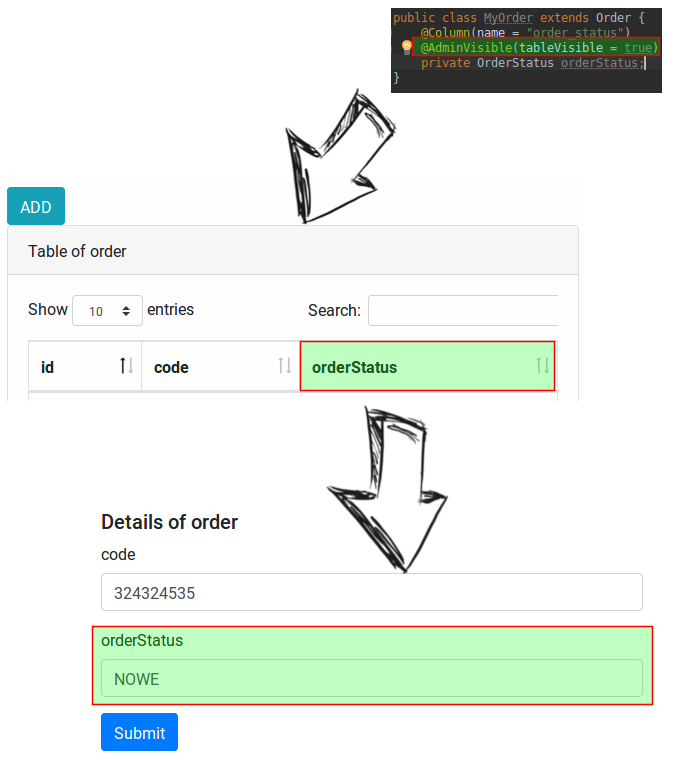
\includegraphics[scale=0.2]{nadpisanieKlasNaPolaWAdminie.png}
			\end{center}
			\caption{{\color{black}Nadpisanie klasy i dodanie własnego pola oraz wyświetlenie go w panelu administracyjnym}} 
		\end{figure}
	\end{column}
\end{columns}
\end{frame}

\begin{frame}{Panel administracyjny}{Zarządzanie relacjami encji}

	\begin{figure}
		\begin{center}
			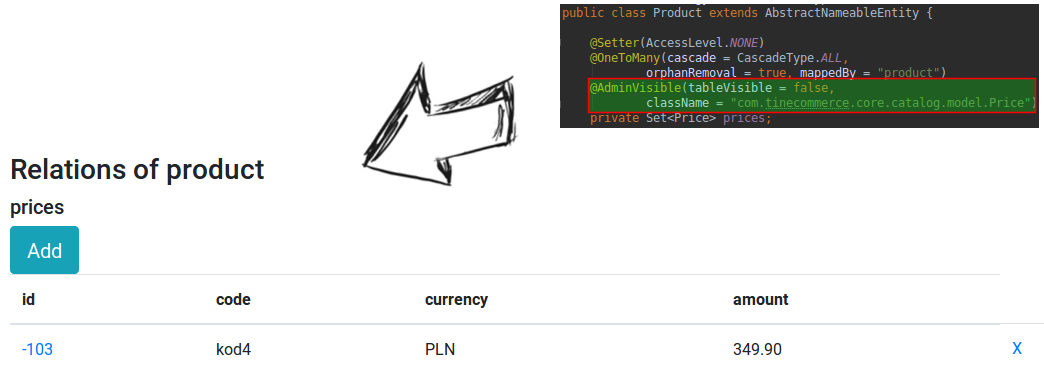
\includegraphics[scale=0.25]{relacjeWDFE.png}
		\end{center}
		\caption{{\color{black}Wygenerowanie komponentu do zarządzania cenami w produkcie}} 
	\end{figure}
\begin{itemize}
	\item<1-> adnotacja \texttt{@AdminVisible} odpowiada również za wyświetlanie relacji w dynamicznym formularzu edycji. 
	\item<1-> obsugiwane są relacje OneToMany jak i ManyToMany
	\item<1-> wyświetlane relacje można dowolnie modyfikować, usuwać lub dodawać
\end{itemize}
\end{frame}


\subsection{Funkcjonalności budowane w platformę}

\begin{frame}{Funkcjonalności systemu}{System klasyfikacyjny}
	\begin{figure}
		\begin{center}
			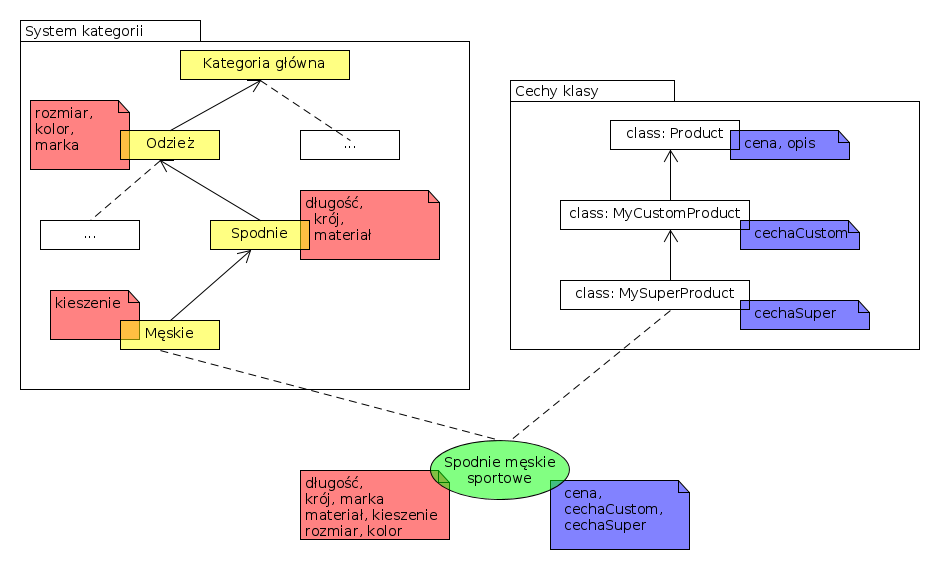
\includegraphics[scale=0.3]{cechyProd.png}
		\end{center}
		\caption{{\color{black}Diagram przykładowy pochodzenia atrybutów produktu}} \label{cechyProd}
	\end{figure}
\end{frame}



\begin{frame}{Funkcjonalności systemu}{Mechanizm indeksująco-wyszukujący}
\begin{itemize}
	\item<1-> do zapytań związanych z katalogiem produktowym użyto serwer Apache Solr 7.5 oparty na silniku Lucene
	\item<1-> Solr umożliwia analizę danych tekstowych: podświetlanie, podpowiadanie i facetowanie 
	\item<1-> obsługa zapytań pochodzących ze sklepu obsługiwana jest przez zewnętrzny serwer, co umożliwia jego skalowanie
	\item<1-> co 15 minut uruchamiany jest job w systemie, który synchronizuje bazę relacyjną z Solrem - indeksacja
	\item<1-> indeksacja to wydobycie atrybutów wyszukiwalnych i facetowalnych z produktu
\end{itemize}
\end{frame}

\begin{frame}{Funkcjonalności systemu}{Przykład działania systemu klasyfikacyjnego z mechanizmem wyszukiwania}
	\begin{figure}
		\begin{center}
			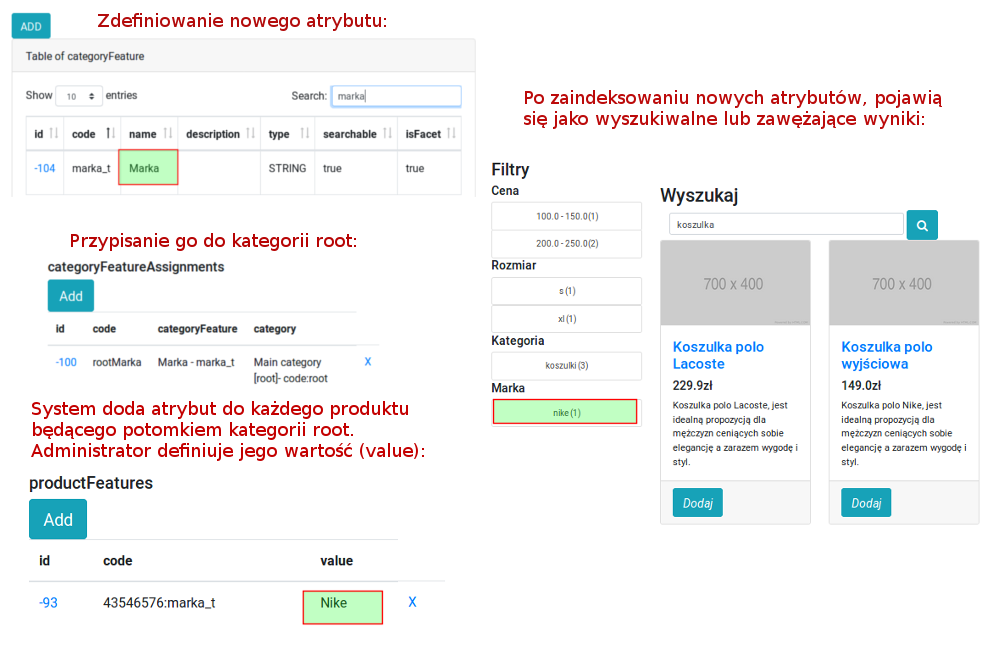
\includegraphics[scale=0.3]{sysklas-wyszfacet.png}
		\end{center}
		\caption{{\color{black}Działanie systemmu klasyfikacyjnego z wyszukiwarką}} 
	\end{figure}
\end{frame}


\begin{frame}{Funkcjonalności systemu}{System uprawnień w panelu administracyjnym}
\begin{itemize}
	\item<1-> użytkownik administracyjny będzie miał kolekcję uprawnień
	\item<1-> struktura systemu uprawnień będzie podobna do struktury kategorii, uprawnienia będą mogły po sobie dzidziczyć
	\item<1-> AdminMenuGroup i AdminMenuItem będą miały kolekcje encji 'uprawnienie', podczas \textit{renderu} menu, będą brane pod uwagę, względem tego, kto jest aktualnie zalogowany
\end{itemize}
\end{frame}

\begin{frame}{Funkcjonalności sklepu}{Inne funkcjonalności, które zostały zaimplementowane z pomocą frameworka}
\begin{itemize}
	\item<1-> koszyk
	\item<1-> możliwość dokonania zakupu
	\item<1-> strona szegółowa produktu
	\item<1-> strona wyszukiwania produktu
	\item<1-> zarządzanie zamówieniami/użytkownikami/adresami 
\end{itemize}
\end{frame}

\begin{frame}
\begin{figure}
	Dziękuje za uwagę
\end{figure}
\end{frame}




\end{document}
